\documentclass[fleqn]{article}
\usepackage[utf8]{inputenc}
\usepackage[margin=2.5cm]{geometry}

% bibliography
\usepackage[round, sort&compress]{natbib}
\usepackage{har2nat}
\bibliographystyle{agsm}

% custom header/footer
\usepackage{fancyhdr}
\pagestyle{fancy}
\renewcommand{\headrulewidth}{0pt}
\fancyhf{}
\rfoot{\textsf{\thepage}}
\lfoot{\textsf{Suzie Brown}}

% miscellaneous formatting
\usepackage{xcolor}
\usepackage[font=small]{caption}
\usepackage{subfig}

% tikz
\usepackage{tikz}
\usetikzlibrary{positioning}

% pseudocode
\usepackage{algorithm}
\usepackage{algorithmicx}
\usepackage{algpseudocode}

% maths
\usepackage{amsmath}
\usepackage{amssymb}
\usepackage{amsthm}
\newtheorem{corollary}{Corollary}
\theoremstyle{definition}
\newtheorem{defn}{Definition}

% useful math symbols
\newcommand{\PR}{\mathbb{P}}
\newcommand{\E}{\mathbb{E}}
\newcommand{\V}{\operatorname{Var}}
\newcommand{\eqdist}{\overset{d}{=}}
\newcommand{\I}[1]{\mathbb{I}\{#1\}}
\newcommand{\Ntoinfty}{\overset{N\to\infty}{\longrightarrow}}
\newcommand{\limNtoinfty}{\underset{N\to\infty}{\lim}}
\newcommand\indep{\protect\mathpalette{\protect\independenT}{\perp}}
\def\independenT#1#2{\mathrel{\rlap{$#1#2$}\mkern2mu{#1#2}}}

% distributions
\newcommand{\Cat}{\operatorname{Categorical}}
\newcommand{\Unif}{\operatorname{Uniform}}
\newcommand{\Mn}{\operatorname{Multinomial}}
\newcommand{\Bin}{\operatorname{Binomial}}

% project-specific commands
\newcommand{\F}{\mathcal{F}_{t-1}}
\newcommand{\vt}[2][t]{v_{#1}^{(#2)}}
\newcommand{\wt}[2][t]{w_{#1}^{(#2)}}
\newcommand{\wbar}[2][t]{\bar{w}_{#1}^{(#2)}}
\newcommand{\vttilde}[2][t]{\tilde{v}_{#1}^{(#2)}}

\title{Comparing expected coalescence rates for multinomial \& residual resampling}
\author{Suzie Brown}
\date{\today}

\begin{document}
\maketitle
\thispagestyle{fancy}

\section*{Case $N=2$}
We can calculate the expected coalescence rates explicitly. With only $N=2$ particles, the coalescence rate becomes
\begin{equation*}
\E[c_N(t) |\F] = \frac{1}{(N)_2} \sum_{i=1}^{N} \E\left[ (\vt{i})_2 |\F \right] 
= \PR[\vt{1} = 0] + \PR[\vt{1} = 2]
\end{equation*}
For residual resampling,
\begin{equation*}
\E[c_2^r(t) |\F] = \I{\wt{1} > 1/2} (2\wt{1} -1) + \I{\wt{1} < 1/2} (2\wt{2} -1)
\end{equation*}
And for multinomial resampling,
\begin{align*}
\E[c_2^m(t) |\F] &= (\wt{1})^2 + (\wt{2})^2 \\
&= \I{\wt{1} > 1/2} ((\wt{1})^2 + (\wt{2})^2) + \I{\wt{1} < 1/2} ((\wt{1})^2 + (\wt{2})^2) \\
&\geq  \I{\wt{1} > 1/2} (\wt{1})^2 + \I{\wt{1} < 1/2} (\wt{2})^2
\end{align*}
Then since $(\wt{i} -1)^2 = (\wt{i})^2 -2\wt{i} +1 \geq 0$, we have that $(\wt{i})^2 \geq 2\wt{i} -1$ and hence we can conclude
\begin{equation*}
\E[c_2^m(t) |\F] \geq \E[c_2^r(t) |\F].
\end{equation*}

\centering
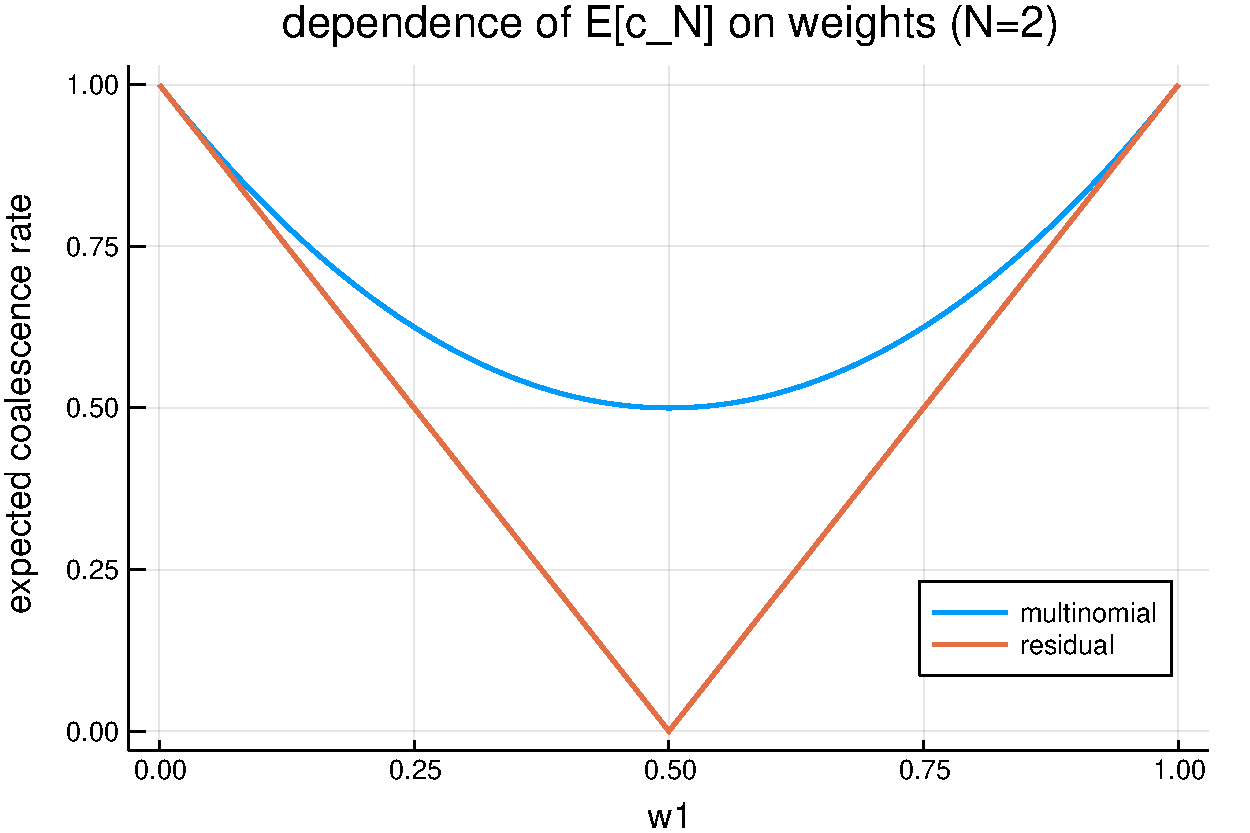
\includegraphics[width=0.8\textwidth]{EcN_mn_res_N2.pdf}

\end{document}